\documentclass[runningheads]{llncs}

\usepackage[T1]{fontenc}
\usepackage{graphicx}
\usepackage{hyperref}
\usepackage{booktabs}
\usepackage{amsmath}

\graphicspath{{../results/}}

\begin{document}

\title{TextFlappyBird: GLIE MC Control \& SARSA($\lambda$)}
\author{Adonis JAMAL\inst{1, 2}}
\institute{CentraleSup\'elec, MDS-MMF \and \'Ecole Normale Sup\'erieure Paris-Saclay, MVA}

\maketitle

\begin{abstract}
    We implement and compare two tabular reinforcement learning agents on the Text Flappy Bird environment: a first-visit GLIE Monte-Carlo control agent and a SARSA($\lambda$) agent with accumulating eligibility traces. Hyperparameters are selected via grid search. SARSA($\lambda$) achieves perfect greedy play, while MC learns a reasonable but high-variance policy. A generalization study reveals that both agents degrade sharply on harder configurations. Code: \href{https://github.com/adonis107/MDS-RL/tree/main/individual\%20assignment}{github.com/adonis107/MDS-RL}.
    \keywords{Reinforcement Learning \and Monte-Carlo Control \and SARSA($\lambda$)}
\end{abstract}

\section{Introduction}
Text Flappy Bird (TFB)~\cite{tfb} is a text-based Gymnasium environment where the agent controls a bird navigating through pipe gaps by choosing to flap or idle ($a \in \{0, 1\}$). We use \texttt{TextFlappyBird-v0}, which returns a compact state $(x_\text{dist}, y_\text{dist})$ representing the distance to the nearest pipe gap centre. This low-dimensional representation makes tabular methods directly applicable. We implement two agents: a first-visit GLIE Monte-Carlo (MC) control agent and a SARSA($\lambda$) agent with accumulating eligibility traces~\cite{sutton2018}.

\section{Methods}
All experiments use \texttt{TextFlappyBird-v0} with training configuration \texttt{height=15}, \texttt{width=20}, \texttt{pipe\_gap=4}, $\gamma = 0.99$. The reward is $+1$ per survived step; greedy evaluation episodes are capped at 5\,000 steps.

\paragraph{GLIE Monte-Carlo Control.} The agent maintains a Q-table updated via the incremental-mean first-visit rule:
\begin{equation}
    Q(s,a) \leftarrow Q(s,a) + \frac{1}{N(s,a)}\bigl(G_t - Q(s,a)\bigr).
\end{equation}
Three epsilon-decay schedules are considered: \emph{linear} ($\epsilon \leftarrow \epsilon_{\max} - k\delta$), \emph{inverse} ($\epsilon = 1/k$), and \emph{exponential} ($\epsilon = \epsilon_{\min} + (1 - \epsilon_{\min})e^{-\lambda k}$), where $k$ is the episode number. Strictly, GLIE requires $\epsilon_k \to 0$; only the inverse schedule satisfies this exactly. Our best configuration uses exponential decay with $\epsilon_{\min}=0.05>0$, which relaxes GLIE to ensure continued exploration. Convergence is therefore not theoretically guaranteed, though the agent still learns an effective policy in practice.

\paragraph{SARSA($\lambda$).} The agent performs online TD updates with accumulating eligibility traces (Section~12.7 of~\cite{sutton2018}):
\begin{align}
    \delta_t &= R_{t+1} + \gamma\, Q(S',A') - Q(S,A), \quad E(S,A) \leftarrow E(S,A) + 1, \\
    \forall (s,a):\quad &Q(s,a) \leftarrow Q(s,a) + \alpha\,\delta_t\,E(s,a), \quad E(s,a) \leftarrow \gamma\,\lambda\,E(s,a).
\end{align}
Traces below $10^{-6}$ are pruned. Exploration follows the inverse schedule $\epsilon = \max(\epsilon_{\min},\, 1/k)$.

\paragraph{Grid Search.} Hyperparameters are selected via parallel grid search (10\,000 training episodes, 500 greedy evaluation episodes). For MC: decay type, decay parameter, and $\epsilon_{\min} \in \{0.01, 0.05\}$ (10 configs). For SARSA: $\alpha \in \{0.05, 0.1, 0.2\}$, $\lambda \in \{0.6, 0.8, 0.9\}$, and $\epsilon_{\min} \in \{0.01, 0.05\}$ (18 configs). The best configuration is then trained for 50\,000 episodes.

\section{Results}
\paragraph{Grid Search.} The MC grid search (Fig.~\ref{fig:mc_gs}) selects exponential decay ($\lambda=0.0005$, $\epsilon_{\min}=0.05$). Exponential decay dominates; fast linear decay ($\text{step}=0.005$) performs poorly as exploration ends prematurely.

For SARSA (Fig.~\ref{fig:sarsa_gs}), the best configuration is $\alpha=0.1$, $\lambda=0.6$, $\epsilon_{\min}=0.05$. Higher $\alpha$ values ($0.1$--$0.2$) consistently outperform lower ones at $\epsilon_{\min}=0.05$, and $\alpha=0.1$ provides the best speed-stability balance.

\paragraph{Training and Evaluation.} Greedy evaluation over 1\,000 episodes after full training is reported in Table~\ref{tab:eval}. SARSA($\lambda$) achieves perfect greedy play, while MC has high variance with frequent early failures (Fig.~\ref{fig:comparison}). The training curves (Figs.~\ref{fig:mc_curves},~\ref{fig:sarsa_curves}) show SARSA converging faster and more smoothly (average training reward $\sim$200 vs.\ $\sim$120 for MC), as eligibility traces propagate credit within each episode rather than waiting for termination. Training-time rewards are lower than greedy evaluation because exploration ($\epsilon > 0$) forces suboptimal actions.

\paragraph{State-Value Functions.} Fig.~\ref{fig:svf} shows $V(s) = \max_a Q(s,a)$ for each agent. Both assign the highest values near the gap centre ($y_\text{dist} \approx 0$), with lower values at extreme offsets. SARSA's value surface is smooth and uniformly high in the safe region. MC exhibits low-value pockets, particularly at moderate $x_\text{dist}$ with $|y_\text{dist}|\geq 2$: these states are visited infrequently yet appear early in long episodes, so their Q-values receive few first-visit updates, each based on high-variance full returns. This directly explains MC's occasional greedy failures (min reward $= 18$ in Table~\ref{tab:eval}): encountering a poorly estimated state triggers a suboptimal action cascade ending in a crash.

\paragraph{Configuration Generalization.} Both agents are evaluated on modified configurations, varying one parameter at a time (Fig.~\ref{fig:generalization}). \textbf{Pipe gap} has the strongest effect: near-perfect scores for gap $\geq 4$ but collapse at gap $= 2$ (MC: 14, SARSA: 31). \textbf{Height/Width} beyond training values also degrades performance, as novel states are unseen during training. The 2D heatmap (Fig.~\ref{fig:heatmap}) confirms difficulty rises steeply as pipe gap shrinks and height increases.


\section{Discussion}
\paragraph{Agent Comparison.}
MC updates Q-values only at episode end using full returns: states visited early in long episodes receive delayed, high-variance corrections, explaining the low-value pockets in Fig.~\ref{fig:svf} and greedy failures (min $= 18$). SARSA($\lambda$) updates online at every step via eligibility traces, so even states encountered once mid-episode receive immediate credit, yielding a smoother value surface and zero-variance greedy play. The trade-off is that SARSA introduces hyperparameters ($\alpha$, $\lambda$); in particular, higher $\alpha$ ($0.1$--$0.2$) performs best because ongoing $\epsilon$-greedy exploration injects noise into returns, and a larger step-size allows the agent to correct for this noise more quickly.

\paragraph{Environment Versions and Transferability.}
\texttt{TextFlappyBird-v0} returns a compact 2D state $(x_\text{dist}, y_\text{dist})$, yielding $\sim$1\,000 tabular entries. \texttt{TextFlappyBird-screen-v0} returns the full $20{\times}15$ character grid, producing a combinatorially vast state space requiring function approximation. The simple variant discards information beyond the nearest pipe (e.g., upcoming gaps, velocity). Transferring to the pixel-based Flappy Bird~\cite{flappybird} would require a DQN-style pipeline~\cite{mnih2015}: stacking consecutive frames to capture velocity, a convolutional encoder to extract spatial features, an experience replay buffer for sample efficiency, and a target network to stabilise bootstrapped updates.

\paragraph{Configuration Generalization.}
Both agents generalise to easier configurations but fail on harder ones (Fig.~\ref{fig:generalization}), as tabular methods cannot interpolate to unseen states. Training on a harder configuration could improve robustness at the cost of longer training.

\paragraph{Limitations.}
The 5\,000-step evaluation cap means SARSA's apparent perfection may mask subtle policy flaws visible only over longer horizons. Grid search with 10\,000 episodes is a rough proxy: the ranking may shift at 50k. Both agents rely on exact state matching with no interpolation, so even minor environment changes introduce unseen states.


\section{Conclusion}
SARSA($\lambda$) learns an optimal policy for TFB, achieving perfect greedy play thanks to online trace-based credit assignment. MC learns a functional but unreliable policy (mean reward $1\,860$ vs.\ the $5\,000$-step cap), as its episode-end batch updates leave many state-action values insufficiently corrected. Neither agent generalises to harder configurations, highlighting the fundamental limitation of tabular methods when the state space varies across settings.


\bibliographystyle{splncs04}
\bibliography{bibliography}


\clearpage
\appendix
\section*{Appendix}
\begin{table}[h]
\centering
\caption{Greedy evaluation after 50\,000 training episodes.}\label{tab:eval}
\begin{tabular}{lcc}
\toprule
Metric & MC & SARSA($\lambda$) \\
\midrule
Mean reward & 1\,860 & 5\,000 \\
Std reward & 1\,556 & 0 \\
Min / Max & 18 / 5\,000 & 5\,000 / 5\,000 \\
Q-table entries & 1\,038 & 1\,066 \\
\bottomrule
\end{tabular}
\end{table}

\begin{figure}[h]
\centering

\includegraphics[width=\textwidth]{MC/gridsearch_results.png}
\caption{MC grid search results. Left: top configurations by mean greedy reward. Right: reward distribution by decay type.}\label{fig:mc_gs}
\end{figure}

\begin{figure}[h]
\centering

\includegraphics[width=\textwidth]{SARSA/gridsearch_results.png}
\caption{SARSA($\lambda$) grid search results. Left: top configurations by mean greedy reward. Right: reward distribution by trace decay $\lambda$.}\label{fig:sarsa_gs}
\end{figure}

\begin{figure}[h]
\centering
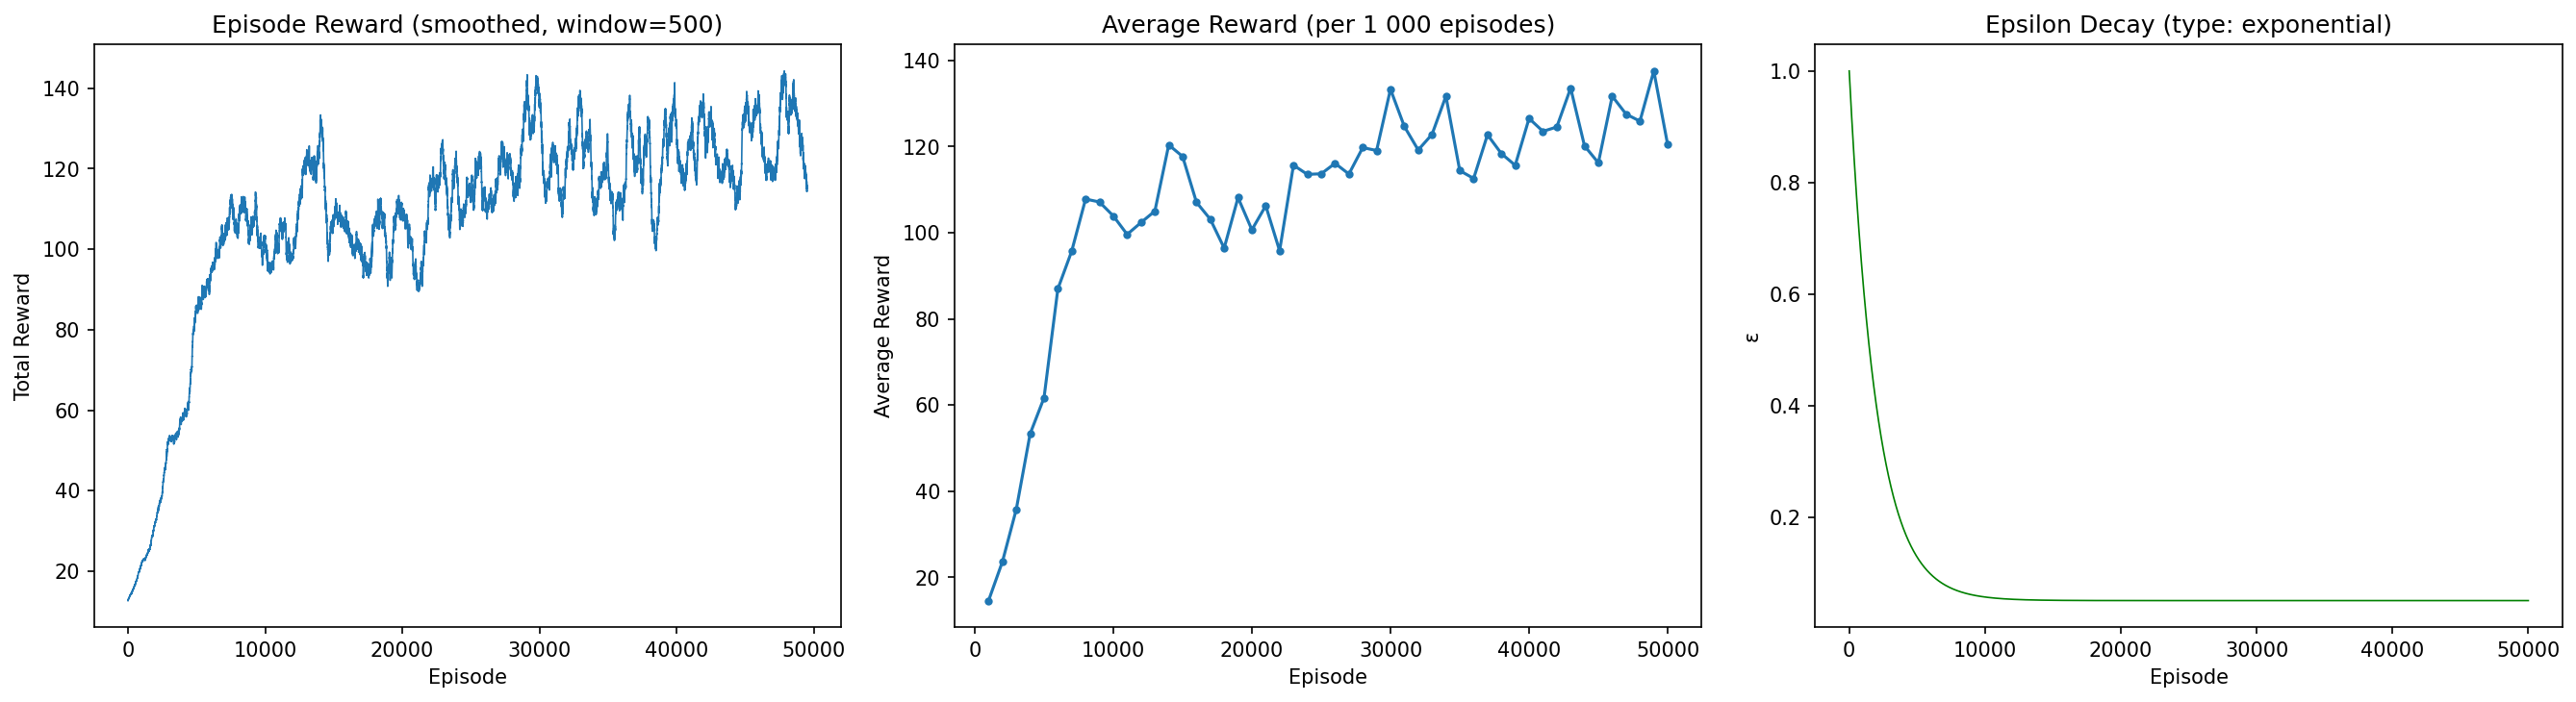
\includegraphics[width=\textwidth]{MC/training_curves.png}
\caption{MC training curves over 50\,000 episodes.}\label{fig:mc_curves}
\end{figure}

\begin{figure}[h]
\centering

\includegraphics[width=\textwidth]{SARSA/training_curves.png}
\caption{SARSA($\lambda$) training curves over 50\,000 episodes.}\label{fig:sarsa_curves}
\end{figure}

\begin{figure}[h]
\centering

\includegraphics[width=0.85\textwidth]{mc_vs_sarsa_comparison.png}
\caption{Overlaid greedy reward distributions (1\,000 episodes each).}\label{fig:comparison}
\end{figure}

\begin{figure}[h]
\centering
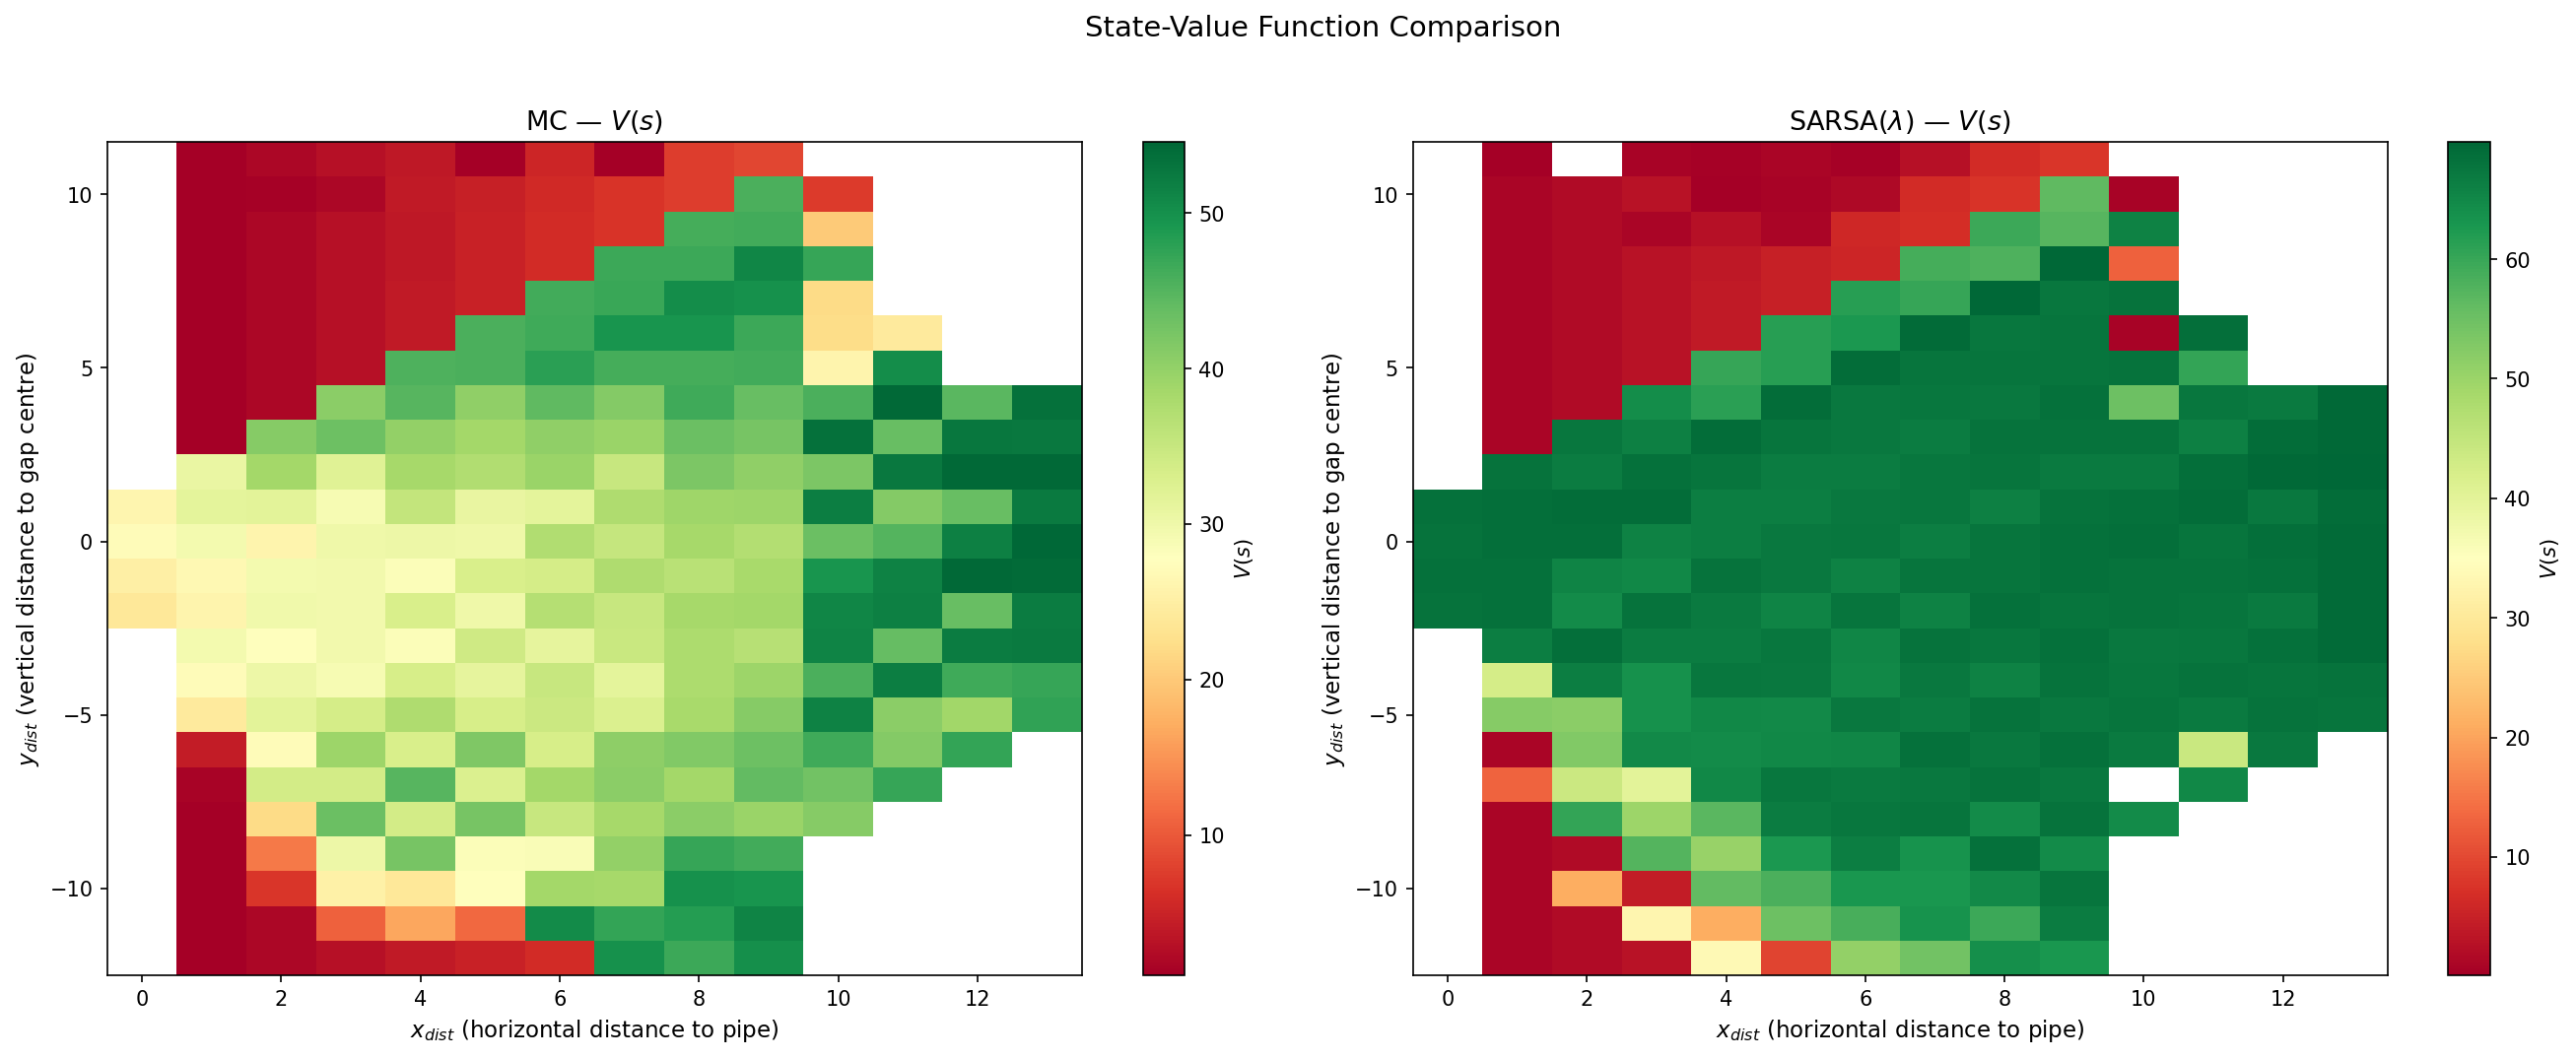
\includegraphics[width=\textwidth]{state_value_comparison.png}
\caption{State-value function $V(s) = \max_a Q(s,a)$ for both agents. States near the gap centre ($y_\text{dist} \approx 0$) have the highest values.}\label{fig:svf}
\end{figure}

\begin{figure}[h]
\centering

\includegraphics[width=\textwidth]{Configurations/generalization.png}
\caption{Mean greedy reward when varying one environment parameter. Dashed line: training value.}\label{fig:generalization}
\end{figure}

\begin{figure}[h]
\centering

\includegraphics[width=\textwidth]{Configurations/heatmap.png}
\caption{2D heatmap of mean greedy reward across pipe gap and height (width fixed at 20).}\label{fig:heatmap}
\end{figure}

\end{document}
